\documentclass[11pt, a4paper]{article}

\usepackage[T1]{fontenc}
\usepackage[utf8]{inputenc}

\usepackage[english]{babel} %Hyphenation, titles, captions, tables in English (for more languages please refer to the babel manual)
\usepackage{csquotes} % Needed by babel
\usepackage{graphicx} %To include graphics
\usepackage{float} %Allows drawing of border around float - also used to define new float environments
\usepackage{endnotes} %Endnotes - footnotes that appear at the end.
\usepackage{pifont} %Font for picture symbols

\usepackage{booktabs}  %booktabs allows \toprule, \midrule, \bottomrule.
\usepackage{threeparttable} % threeparttable allows table notes, and adjusting the width of the caption to the width of the table


% With the next 3 parameters you can control the behaviour of latex how it handles floats and text. Normally it is not possible to fill a single page with only floats because LaTeX tries to achieve a certain text/float ratio per page. With these paremters this can be changed.

\renewcommand{\textfraction}{0.001} % having very little text on a page is OK
\renewcommand{\topfraction}{0.999}  % Having many floats in the upper half is OK
\renewcommand{\bottomfraction}{0.999} % Having many floats in the lower half is OK

% The omnipotent drawing package
\usepackage{tikz}

% Math packages
\usepackage{amsmath} 
\usepackage{amsfonts}
\usepackage{amssymb}

% Change page dimensions/borders
\usepackage[top=2.5cm, left=2cm, right=2.5cm, bottom=2cm]{geometry}
\usepackage{a4}

% Index directory
\usepackage{makeidx}
\makeindex

% Bibliography packages
\usepackage[style=authoryear, backend=biber, maxnames=5]{biblatex}
\addbibresource{bibliography.bib}



\pagestyle{headings} %standard headings. other options: plain, empty


% Custom command
\newcommand{\ltx}{\LaTeX}

%\linespread{1.2}\selectfont % Global Zeilenabstände ändern

\setlength{\belowcaptionskip}{2ex}
\setlength{\abovecaptionskip}{1ex}

% Redefinition of margin parameters
% More information: http://tex.stackexchange.com/questions/48571/redefine-marginpar-with-renewcommand
\let\oldmarginpar\marginpar
\renewcommand{\marginpar}[1]{\oldmarginpar{\textit{#1}}}




% Title page
\title{\ltx{} made easy}
\author{John Doe\\ University Here\thanks{hans.musterman@uni-here.edu} \and Michael Smith\\University there\thanks{peter.lustig@uni-there.edu}}

% Should be loaded last to avoid overwriting of package settings
\usepackage{hyperref} %Creates clickable references in the document - ideally loaded last in the document preambel

%%%%%%%% BEGIN OF DOCUMENT %%%%%%%%
\begin{document}

\maketitle
\tableofcontents
\newpage

\section{Easier than its reputation}

For a ``simple'' \ltx-document only a handful of commands are needed. You do not even have to care aboutr formatting but can instead completely focus on the text.

Apart from a few special characters, the majority of the text can be typed as you usually do.

\section{Simple text formatting}

A new paragraph can be produced if you insert at least one empty line. It does not matter whether it is one or many empty lines it all ends up creating just a simple new paragraph. So unlike in Word you can not format your documents with many new lines. Same applies to spaces: one or many spaces always only insert a simple space.

\subsection{Hyphenation and dashes}

You do not have to care about hyphenation. \ltx\ will take care of this. However if there is a word that you want to have hyphenated differently, there are options to achieve this.

There are different types of dashes. The normal dash (-) -- used to connect words -- and the so called \textit{Halbgeviertstrich}: -- which is just 2 consecutive dashes or the long version of this (---) (3 consecutive dashes).


\subsection{Anführungen}
Quotation marks\index{Quotations} are normally set with \`{}\`{} \verb+''+ (`` ''). For German quotes use "\`{} "\verb+'+ ("` "') or for French \verb+"< ">+ ("< ">).

\begingroup
\setlength{\parindent}{0pt}
\setlength{\parskip}{1.5ex plus 0.5ex minus 0.2ex}
\section{Text formatting\label{sec:eftf}}

\subsection{Characters}

\subsubsection{Special characters}
If you want to use non ASCII characters (like é or ł ą ę) it is recommended to use UTF8 encoded input and a font that also supports these characters (most fonts support characters used in French, Polish, Italian and others). This is also why the document loads \texttt{fontenc} and \texttt{inputenc} with the option \texttt{T1} and \texttt{utf8} respectively.

\subsection{Paragraphs}
This text contains both paragraphs and simple new lines. For section \ref{sec:eftf} (starting on page \pageref{sec:eftf}) it has been set that for the first line of every paragraph there is no indentation.

\begingroup
\raggedright % Left justified
The spacing between paragraphs should be 1.5ex, can be extended at most by 0.5ex and reduced by at most 0.2ex. This paragraph and the next should be left justified. 

\vspace{1cm}
\subsection{Misc.} 
An \fbox{additional} $1$\,cm has been inserted before this paragraph.
\endgroup
\endgroup

\section{Visual formatting}
Most of the formatting done in section~\ref{sec:eftf} \nameref{sec:eftf} are of visual nature i.e. the commands describe how the text should look like. For all practical purposes you ideally should not use these kinds of commands (of course there are justified exceptions). Better is it to use logical formatting which describes which significance a certain part of the text has with respect to the document structure or its content.

\section{Fonts in \ltx}

The font style in \ltx{} is defined by 3 features:

\begin{enumerate}
\item Font family
\begin{itemize}
\item Fonts with serifs (roman): proportional fonts with small helper lines attached to each letter.
\item \textsf{Sans serif fonts: proportional fonts without helper lines}.
\item \texttt{Typewriter fonts: monospaced font}.
\end{itemize}
\item Font weight:
\begin{itemize}
\item normal weight
\item \textbf{bold weight\index{fett|textbf}}
\end{itemize}
\item Form of the font:
\begin{itemize}
\item Upright fonts
\item \textsl{Slanted fonts}
\item \textit{Italic fonts}
\item \textsc{Small caps}
\end{itemize}
\end{enumerate}

Even though there are many options to manipulate font face, weight and style there is one rule you should always remember:
\begin{quote}
Typography is a trade that has to be learned. Someone not trained in this often makes disastrous mistakes. Many people mistakenly believe that the design of a text is mostly aestethics and a ``nice look'' is the ultimate goal -- which is a mistake. A text is to be read and not to be wondered at in a museum. Readability and intelligibility are much more important than the ``nice looks''.
\end{quote}

\noindent Here a few pointers that you should consider when you write your text:
\begin{itemize}
\item[\ding{43}] Extensive texts should be set with a serif font.
\item[\ding{43}] Highlighting in a text can be done with slanted or italic form. Italic fonts highlight better than slanted. Really important parts can be highlighted with bold faced text.
\item[\ding{43}]  \textsf{Text sans serif are suitable for headers and titles}
\item[\ding{43}] Less is more: Do not try to overdesign your text. Leave most work to \ltx.
\end{itemize}


\begin{table}[t]
\caption{Example table  \label{tab:Schriftgroessen}}
\centering
\begin{tabular}{lccc}
\toprule
\textbf{\ltx-Command} & \multicolumn{3}{c}{\textbf{Base size}}\\
\cline{2-4} & \textbf{10pt} & \textbf{11pt} & \textbf{12pt}\\
\midrule
\midrule
\verb+\tiny+			& 5pt & 6pt 	& 6pt\\
\verb+\scriptsize+		& 7pt & 8pt		& 8pt\\
\verb+\footnotesize+	& 8pt & 9pt		& 10pt\\
\verb+\small+			& 9pt & 10pt	& 11pt\\
\midrule
\midrule
\verb+\normalsize+		& 10pt	& 11pt	& 12pt\\
\midrule
\midrule
\verb+\large+			& 12pt	& 12pt	& 14pt\\
\verb+\Large+			& 14pt	& 14pt	& 17pt\\
\verb+\LARGE+			& 17pt	& 17pt	& 20pt\\
\verb+\huge+			& 20pt	& 20pt	& 25pt\\
\verb+\Huge+			& 25pt	& 25pt	& 25pt\\
\bottomrule
\end{tabular}
\end{table}%

\section{Table example}
Table \ref{tab:Schriftgroessen} shows the font size for the \ltx font size commands with respect to their base font size.

The smallest font size is 5~pt the largest 25~pt.

\section{Images in \ltx}
\ltx{} allows the creation of graphics directly with \ltx commands as embedding external image files. Both option will be shown in the following examples.

\subsection{Line figures with \ltx commands}

\ltx{} allows the creation of plots directly via \ltx-commands. One example can be seen in fig.~\ref{fig:tikz}. Tikz is an additional package like many which has to be loaded in the
preamble. With Tikz one has endless possibilities, all you need is an idea how to put it to paper. For more information please read \textit{A very minimal introduction to Tikz} (\url{http://cremeronline.com/LaTeX/minimaltikz.pdf}).
%
\begin{figure}[t]
\centering
\begin{tikzpicture}[scale=0.6]
% Create coordinate system
\draw [->] (-5,0) -- (5,0);
\draw [->] (0,-5) -- (0,5);

% Label axis
\node [below] at (5,0) {$x$};
\node [left] at (0,5) {$y$};

% Repeat vertical line in the 1. quadrant
\foreach \x in {0.25, 0.5, 0.75,...,3} {
\draw (\x, 0) -- (\x, 3);
}

% The rectangle: cycle connects the last point with the first.
\draw (-3,-3) -- (-3,3) -- (3,3) -- (3,-3) -- cycle;

% Diagonal line
\draw (-4,-4) -- (4,4);

% Separation of the coordinate axis
\foreach \t in {-4,-3,...,4}{
\draw (\t, -0.2) -- (\t, 0.2);
\draw (-0.2,\t) -- (0.2,\t);
}
\end{tikzpicture}
\caption{A Tikz figure\label{fig:tikz}}
\end{figure}


\subsection{Some history -- embedding of pictures}
In the beginning there was a book project. IT professor Donald Knuth typeset the first volume of his book ``The Art of Computer Progrmaming'' 1969 with \textit{Monotype} a technology from the 19\(^{\text{th}}\) century. In 1976 when the second volume was about to be published, most of the monotype technology has been replaced by photographic typesetting. When Knuth received the pages to proofread he thought them to be awful and thus he began in 1977 to write his own typesetting system -- \TeX was born.

\begin{figure}[htb]
\centering
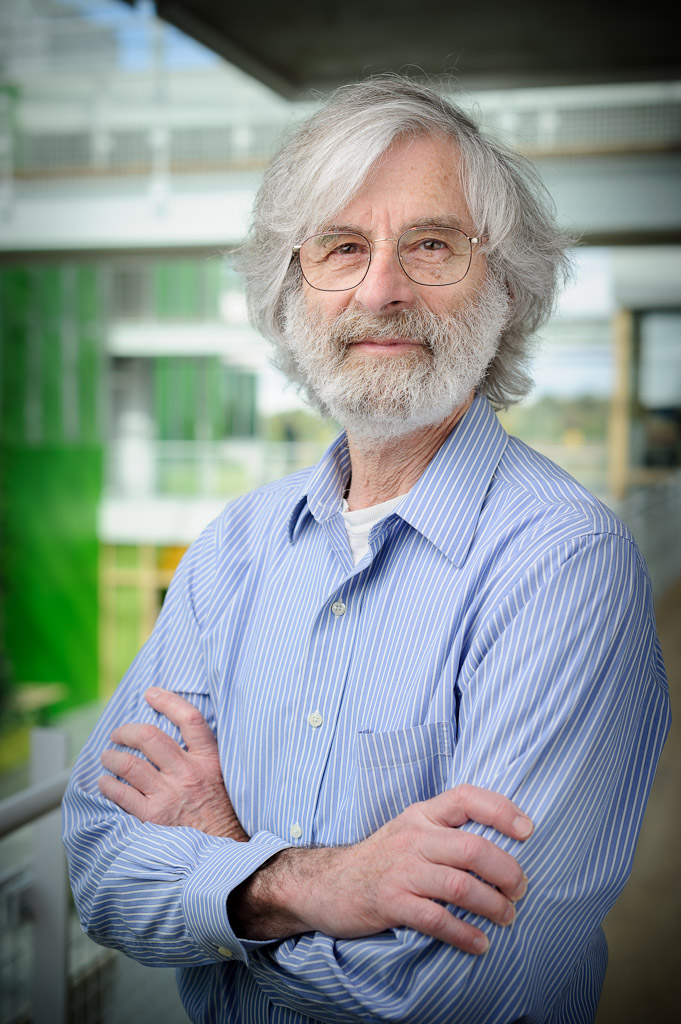
\includegraphics[width=0.3\textwidth]{Leslie_Lamportd}
\caption{Leslie Lamport\label{fig:LL}}
\end{figure}

\TeX{} offers many option for text formatting but it is difficult and cumbersome to use. Leslie Lamport, an American computer scientist believed that an author should focus on content and not formatting. In 1984 he began writing a macro package for \TeX{} which takes responsibility for many formatting decisions and many other simplifications -- \ltx.

\section{Basics of math typesetting}

Scientific papers with a lot of formulas set a high requirement to the typesetting system because mathematical expressions and formulas should be treated differently that running text. One emphasis of the development of \TeX{} and \ltx{} was on a high-quality for the mathematical typesetting to be in accordance with the conventions.

\begingroup
\floatstyle{boxed}
\restylefloat{figure}
\begin{figure}[p!] %p erzielt, dass die figure auf einer Seite speziell für floats platziert wird
Given the family of functions
\begin{displaymath}
f_a(x) = \frac{x+a}{x^2}~\mbox{mit } a \in \mathbb{R}
\end{displaymath}
\begin{enumerate}
\item Investigate the family of functions \( f_a\) for it's maximum domain \(\mathbb{D}\). Determine the asymptotes for the graphs as the behavious of the graphs at the border of the domain.
\item Proof that for two different graphs of the family there is no intersection but they approach each other arbitrary close at \(x\to\infty\).
\item Draw the graph \(G_{f_1}\) in the range \(I = \left[-4;4\right]\) in a suitable coordinate system.
\item Show that
\begin{displaymath}
F(x) = x +(x+1)\cdot\ln(x+1) - 2x\cdot\mbox{ln}(x)
\end{displaymath}
is a primitive of \(\displaystyle g(x) = \ln\left(\frac{x+1}{x^2}\right)\) is.
\end{enumerate}
\caption{A simple maths sheet}
\label{fig:formeln}
\end{figure}
\endgroup

Part of the mathematical typesetting are:
\begin{itemize}
\item Numbers, variables and operators
\item Mathematical symbols
\item Name of functions
\item Greek letters
\item Indices and exponents
\item Complete mathematical formulas
\item various special characters.
\end{itemize}

Numbers and operators are set in an upright style, variables mostly italic without kerning.

A very important package for typesetting formulas is developed by the American Mathematical Society (\AmS) called \textit{amsmath} which in addition to operators and symbols also offers additional structuring elements and design possibilities. It is a good idea to load this package in any preamble (\verb+\usepackage{amsmath}+).

Fig.~\ref{fig:formeln} shows a selection of formulas. Also it shows that a figure environment is not necessarily only for figures.ht zwingend ein Bild (im technischen Sinne) enthalten sein muss.

\clearpage %beginnt eine neue Seite und platziert alle noch nicht gesetzten Floats

\section{Footnotes and margin notes}

Nachfolgend finden Sie ein Zitat aus dem Lehrbuch, ergänzt durch einige Anmerkungen der Kursautoren -- themabezogen als Fussnoten\marginpar{Fussnoten}:

\begin{quote}
Längere, zusätzliche Erklärungen werden meist nicht im Fliesstext eingefügt, da auf diese Weise schnell der Sinnzusammenhang verloren gehen kann. Stattdessen wird durch eine Markierung -- meist eine kleine hochgestellte Zahl\footnote{Üblicherweise in aufsteigender Reihenfolge.} -- auf sie verwiesen\footnote{Beachten Sie aber, dass auch eine Fussnote den Lesefluss beträchtlich stören kann. Wägen Sie immer ab, ob Sie die Anmerkung wirklich brauchen und ob diese im Fliesstext nicht besser aufgehoben wäre.}. Im Seitenfuss wird diese Markierung wiederholt und der erklärende Text in einer kleinen Schriftgrösse\footnote{Eben in der Grösse \textbackslash\texttt{footnotesize}.} ausgegeben. Zur deutlichen Trennung zwischen dem Fliesstext und den Fussnoten wird zwischen diesen Seitenbereichen eine kurze horizontale Linie mit entsprechendem Leerraum gesetzt\footnote{Es gibt auch Publikationen, wo diese Linie über die ganze Seitenbreite ausgezogen wird.}.

Im Fliesstext können Sie mit \ltx{} relativ einfach Fussnoten anbringen. Die Nummerierung wird dabei automatisch von \ltx{} verwaltet, so dass es auch im Nachhinein möglich ist, Fussnoten neu einzufügen oder zu löschen\footnote{Weiter verwaltet \ltx{} auch die Seite, wo der Fussnotentext erscheint. Dieser sollte immer auf der selben Seite stehen, wie die Fussnotenmarkierung. \ltx{} gelingt dies fast immer (ausser in einigen verzwickten Fällen), wohingegen Microsoft Word hier überdurchschnittlich oft scheitert.}. Die Nummerierung wird mit jedem Kapitel (Dokumentklassen \textit{report} und \textit{book}) wieder zurückgesetzt, so dass die Nummerierung der Fussnoten wieder bei Eins beginnt. Fussnoten können auch innerhalb der \textit{minipage}-Umgebung verwendet werden.

Auf Grund der \ltx-internen Bearbeitung der Fussnoten gibt es einige Dokumentteile, in denen dieser Automatismus nicht korrekt funktioniert: z.B. in Tabellen, Gleitumgebungen, mathematischen Ausdrücken, \ltx-Boxen. In diesen Fällen bedarf es eines Umweges, um dort Fussnoten anzubringen.
\end{quote}

Auch bei Endnoten\marginpar{Endnoten} handelt es sich um erklärende Texte, die im Gegensatz zu Fussnoten aber gesammelt am Ende des Kapitels oder des Dokuments ausgegeben ewrden. Gerade bei längeren Anmerkungen oder vielen Anmerkungen pro Seite kann sich der Einsatz von Endnoten lohnen. \ltx{} benötigt für Endnoten \parencite{lkgt} -- im Gegensatz zu Fussnoten -- ein Zusatzpaket: \texttt{endnotes}. Da Endnoten tendentiell eher seltener als Fussnoten verwendet werden, werden wir in dieser Übung auf Endnoten verzichten.

Marginalien\marginpar{Marginalien} sind in einem gewissen Sinne ebenfalls Anmerkungen. Allerdings handelt es sich dabei nicht um längere, erklärende Texte, sondern eher um Hinweise, um bestimmte Stellen im Text zu kennzeichnen.

\section{Literaturhinweise mit Bib\LaTeX}
Bibliographie-Erstellung mit dem Zusatzprogramm Bib\LaTeX{} bedeutet, dass Sie Ihre Literatur in separaten Textdateien erfassen, welche als Bibliographie- dateien bezeichnet werden. Sie können zur Verbesserung der Übersichtlichkeit separate Bibliographiedateien für verschiedene Themengebiete anlegen.

Die einzelnen Referenzen schreiben Sie in die Dateien im Bib-Format, das eines der meistbenutzten Formate für Bibliographiesammlungen im Textformat ist und auch von anderen Programmen weiterverarbeitet werden kann. Bib-Dateien lassen sich z.B. bequem mit dem Programm "<JabRef"> bearbeiten, welches als Java-Applikation plattformübergreifend verfügbar ist.
Das Programm Bib\LaTeX{} erledigt dann folgende Aufgaben für Sie:
\begin{itemize}
\item Erstellung einer Liste aller im Text zitierter Dokumente
\item Unterstützung für die Hinzunahme weiterer, nicht zitierter Dokumente
\item Auswahl aus verschiedenen Layoutstilen, die Sie auch ändern oder komplett selber schreiben können (was allerdings absolut nicht trivial ist!)
\item Automatische Formatierung der Referenzen gemäss dem gewählten Layoutstil
\item Sortierung der Literaturliste
\item Unterstützung von verschiedenen Referenzformen im Text
\item Syntaxprüfung der Bibliographiedatei
\item Prüfung der Eindeutigkeit von Schlüsseln
\end{itemize}
Mit der Benutzung von Bib\LaTeX{} gewinnen Sie aber mehr als das: Wer Bibliographiedateien im Bib-Format in grossem Ausmass benutzt wird es schnell als gutes Mittel zur Bibliographieverwaltung schätzen lernen. Als textbasiertes System, für das diverse graphische Oberflächen existieren (z.B: "<JabRef">), ist es auch gut zum Nachschlagen oder Austausch mit Kollegen. Da Sie beliebig weitere Felder hinzufügen können, ist es auch geeignet, um z.B. Quellenangaben oder Bibliotheksstandorte zu notieren, Schlüsselwörter zu vergeben, usw.


\section{Indices}
Lassen Sie uns zuerst Leslie Lamport, den Autoren von \ltx{} zum Thema zum Wort kommen:
\begin{quote}
Der Index soll dem Leser helfen, bestimmte Informationen im Dokument zu finden, und zwar so einfach wie möglich. Viele Verfasser indizieren Wörter, indem sie alle Seiten, auf denen ein bestimmter Begriff erscheint, auflisten. Ein guter Autor erstellt einen Index nach Konzepten -- Ideen, Fakten, Personen usw.

Zur Erstellung eines Index müssen Sie sich zunächst überlegen, welche Konzepte Sie dort aufführen wollen. Danach müssen Sie herausfinden, nach welchen Schlagworten sich der Leser vermutlich orientiert, um ein Konzept zu finden. Sie müssen sich überlegen, welche Leserschaft das Buch haben wird, und wie die Leser das Konzept auffassen. Beschränken Sie sich nicht auf die Auflistung der Wörter, die Sie selbst zur Beschreibung des Konzeptes verwendet haben.

Sie sind vielleicht versucht, das Stichwortverzeichnis bereits beim Schreiben des Dokumentes anzulegen. Widerstehen Sie dieser Versuchung. Es ist nahezu unmöglich, auf diese Weise einen guten Index zu erstellen. Fügen Sie beim Schreiben \verb+\index+-Befehle ein, damit Sie sich später daran erinnern, für welche Begriffe Sie Indexeinträge erstellen wollten, aber bereiten Sie sich darauf vor, diese Befehle noch einmal zu überarbeiten, wenn Sie den Index erstellen.
\end{quote}
Nehmen Sie sich diese Aussagen unbedingt zu Herzen\cite{dlb}, denn wie Sie auch an einem kurzen Text schon sehen können, nützt ein Index, wo jedes Vorkommen eines bestimmten Stichwortes aufgelistet wird, nicht sonderlich viel. Trotzdem wollen wir in diesem Beispieltext gleich davon abweichen, denn hier soll es um die Anwendung der Index-Befehle und nicht um das Endresultat gehen.

\begin{table}[h!]
\centering
\caption{Übersicht der Indexierbefehle\label{tab:Indexbefehle}}
\begin{tabular}{lll}
\toprule
Example &	Index Entry	 & Comment\\
\midrule
\verb+\index{hello}+ &	hello, 1	& Plain entry \\
\verb+\index{hello!Peter}+	&  Peter, 3	 &Subentry under 'hello'\\
\verb+\index{Sam@\textsl{Sam}}+&	\textsl{Sam}, 2	&Formatted entry\\
\verb+\index{Lin@\textbf{Lin}}	+&	\textbf{Lin}, 7	&Same as above\\
\verb+\index{Jenny|textbf}+&	Jenny, \textbf{3}	&Formatted page number\\
\verb+\index{Joe|textit}+&	Joe, \textit{5}	&Same as above\\
\verb+\index{ecole@\'ecole}+&	école, 4&	Handling of accents\\
\verb+\index{Peter|see{hello}}+&	Peter, \textit{see} hello	&Cross-references\\
\verb+\index{Jen|seealso{Jenny}}+ &	Jen, \textit{see also} Jenny	&Same as above\\
\bottomrule

\end{tabular}

\end{table}%

\newpage

\printbibliography
\printindex
\end{document}
